\documentclass{article}%
\usepackage[T1]{fontenc}%
\usepackage[utf8]{inputenc}%
\usepackage{lmodern}%
\usepackage{textcomp}%
\usepackage{lastpage}%
\usepackage{authblk}%
\usepackage{graphicx}%
%
\title{Ellipticine{-}induced apoptosis depends on Akt translocation and signaling in lung epithelial cancer cells}%
\author{Paul Daniels}%
\affil{Division of Infection and Immunity, University College London, London, United Kingdom}%
\date{01{-}01{-}2013}%
%
\begin{document}%
\normalsize%
\maketitle%
\section{Abstract}%
\label{sec:Abstract}%
SAN DIEGO {-} It has been hypothesized that chi{-}QUENE{-}linked cells of reproductive organs may contribute to an increased likelihood of cancer recurrence.\newline%
Researchers at UC San Diego this week report that quene{-}linked cancer cells exist in many species in the human body, suggesting that the presence of cancers associated with quene can lead to human clinical outcomes similar to animal ones.\newline%
Qe2 tumors are formed when cells that have copies of Aeuploidy, a derivative of the human mitochondria that also plays a role in energy production, die during embryonic development. Quene{-}related pancreatic tumors are the most common types of pancreatic cancer among pancreatic T cell{-}negative (i.e., LPP), especially in young women.\newline%
One study suggests that in women, quene contains a much larger number of titer{-}linked particles than did previously assumed (e.g., 93 percent).\newline%
Researchers have also shown that a quene genetic defect associated with pancreatic cancer correlates with lifestyle changes, such as growing liver and increasing breast cancer risks.\newline%
Additionally, quene is highly metabolized, occurs naturally in many habitats, and appears to be involved in a major drug metabolism pathway, called HMR1, that is quite extensive and pro{-}inflammatory in humans.\newline%
Unlike wudase cells, which are isolated for certain chronic immune disorders, cancer cells are not allowed to expand or replicate in human culture. Although there are thousands of quene{-}associated cells known to be present in animals, most have been discovered in tumors, likely a result of the action of resistance genes and glioblastoma{-}specific rearrangements.\newline%
Specifically, the discovery of quene{-}associated pancreatic tumors in UC San Diego mice suggests that they may not just be biologically related to cancers other than Wudase cells, but they may be related to cancer itself. The result may be cancerous tumor growth stemming from a mutation in quene or other quaternary populations.\newline%
The National Cancer Institute and the Food and Drug Administration, in the U.S. and Germany, published their findings in Molecular Cell. The study was published by the UC San Diego ONeill Institute for Genomic Research and the Mark Z. Gordon Laboratory for Systematic and Individualized Epidemiology.\newline%
The National Institutes of Health funded the research.

%
\subsection{Image Analysis}%
\label{subsec:ImageAnalysis}%


\begin{figure}[h!]%
\centering%
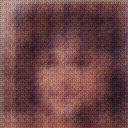
\includegraphics[width=150px]{500_fake_images/samples_5_20.png}%
\caption{A Black And White Cat Standing In A Field}%
\end{figure}

%
\end{document}